\subsection{ViMo-Flow Framework}
\label{subsec:framework}

\subsubsection{Diffusion Formulation}
The denoising process follows a standard Markovian corruption of the clean motion $\mathbf{m}_0$. The forward transitions are defined as
\[
q(\mathbf{m}_t|\mathbf{m}_{t-1})=\mathcal{N}(\sqrt{\alpha_t}\mathbf{m}_{t-1},(1-\alpha_t)\mathbf{I}),
\]
producing $\mathbf{m}_t$ at each step $t$. Unlike the original DDPM parameterization, which predicts the noise term $\boldsymbol{\epsilon}$, the network $D(\mathbf{m}_t,t,\mathbf{p})$ directly outputs an estimate of the clean motion $\hat{\mathbf{m}}_0$. This approach is better suited to the structured output space—6D rotations~\cite{6drot2020}, root translation, and binary contact labels—where predicting noise would require additional post-processing. The training objective minimizes the simple L2 loss
\[
\mathcal{L}_{\text{simple}}=\mathbb{E}[\|\mathbf{m}_0-D(\mathbf{m}_t,t,\mathbf{p})\|^2],
\]
averaged over random timesteps and paired samples. At inference, the posterior mean $\tilde{\boldsymbol{\mu}}_t$ is computed from $\hat{\mathbf{m}}_0$ using the closed-form expression
\[
\tilde{\boldsymbol{\mu}}_t=\frac{\sqrt{\bar{\alpha}_{t-1}}\beta_t}{1-\bar{\alpha}_t}\hat{\mathbf{m}}_0+\frac{\sqrt{\alpha_t}(1-\bar{\alpha}_{t-1})}{1-\bar{\alpha}_t}\mathbf{m}_t,
\]
enabling deterministic DDIM sampling or stochastic DDPM sampling.


%%%%%%%%%%%%%%%%%%%%%%%%%%%%%%%%%%%%%%%%%%%%%%%%%%%%%%%%%%%%%%%%%%%%%

\begin{algorithm}
\caption{Forward Diffusion Sampling}
\label{alg:forward_diffusion}
\begin{algorithmic}[1]
\Require Clean input $\mathbf{x}_0$, timestep vector $\mathbf{t}$, noise schedule $\{\beta_t\}_{t=1}^T$
\Ensure Noisy sample $\mathbf{x}_t$

\State Initialize $\alpha_t = 1 - \beta_t$ for $t = 1,\dots,T$
\State Compute $\bar{\alpha}_t = \prod_{i=1}^{t} \alpha_i$ \Comment{Cumulative product}

\State Sample $\epsilon \sim \mathcal{N}(\mathbf{0}, \mathbf{I})$ with $\text{dim}(\epsilon) = \text{dim}(\mathbf{x}_0)$
\State $\bar{\alpha}_{\mathbf{t}} \leftarrow \text{gather}(\bar{\alpha}, \mathbf{t})$ \Comment{Select $\bar{\alpha}$ values for given timesteps}

\If{$\text{dim}(\mathbf{t}) = 1$}
    \State $\bar{\alpha}_{\mathbf{t}} \leftarrow \text{reshape}(\bar{\alpha}_{\mathbf{t}}, (B, 1, 1))$
\Else 
    \State $\bar{\alpha}_{\mathbf{t}} \leftarrow \text{reshape}(\bar{\alpha}_{\mathbf{t}}, (B, S, 1))$ \Comment{$\text{dim}(\mathbf{t}) = 2$ PTSS case}
\EndIf

\State $\mathbf{x}_t \leftarrow \sqrt{\bar{\alpha}_{\mathbf{t}}} \cdot \mathbf{x}_0 + \sqrt{1 - \bar{\alpha}_{\mathbf{t}}} \cdot \epsilon$
\State \Return $\mathbf{x}_t$
\end{algorithmic}
\end{algorithm}

%%%%%%%%%%%%%%%%%%%%%%%%%%%%%%%%%%%%%%%%%%%%%%%%%%%%%%%%%%%%%%%%%%%%%

\begin{algorithm}
\caption{Reverse Denoising Sampling}
\label{alg:reverse_denoising}
\begin{algorithmic}[1]
\Require Model $\mathcal{M}$, initial state specification $\mathbf{x}_T$, total steps $T$, conditioning input $\mathbf{p}_{2d}$, stochasticity flag $\sigma_{flag}$, noise schedule $\{\beta_t\}_{t=1}^T$
\Ensure Generated motion sequence $\mathbf{x}_0$

\State Initialize $\alpha_t = 1 - \beta_t$ for $t = 1,\dots,T$
\State Compute $\bar{\alpha}_t = \prod_{i=1}^{t} \alpha_i$ \Comment{Cumulative product}

\If {$\mathbf{x}_T$ is dimension tuple}
    \State $\mathbf{x}_t \sim \mathcal{N}(\mathbf{0}, \mathbf{I})$ with shape $\mathbf{x}_T$
\Else
    \State $\mathbf{x}_t \leftarrow \mathbf{x}_T$ \Comment{Clone input tensor}
\EndIf

\State Set batch size $B \leftarrow \text{dim}(\mathbf{x}_t, 0)$
\State $\mathcal{M}.\text{eval}()$ \Comment{Set model to evaluation mode}

\For{$t = T-1$ down to $0$}
    \State $\mathbf{t} \leftarrow \text{vector of length } B \text{ with value } t$ \Comment{Batch timestep vector}
    \State $\hat{\mathbf{x}}_0 \leftarrow \mathcal{M}(\mathbf{x}_t, \mathbf{t}, \mathbf{p}_{2d})$ \Comment{Model prediction}
    
    \If{$t > 0$}
        \State $\bar{\alpha}_t \leftarrow \bar{\alpha}[t]$, $\bar{\alpha}_{t-1} \leftarrow \bar{\alpha}[t-1]$
        \State $c_1 \leftarrow \sqrt{\bar{\alpha}_{t-1}} \cdot \frac{\beta_t}{1 - \bar{\alpha}_t}$
        \State $c_2 \leftarrow \sqrt{\alpha_t} \cdot \frac{1 - \bar{\alpha}_{t-1}}{1 - \bar{\alpha}_t}$
        \State $\boldsymbol{\mu} \leftarrow c_1 \cdot \hat{\mathbf{x}}_0 + c_2 \cdot \mathbf{x}_t$ \Comment{Posterior mean}
        
        \If{$\sigma_{flag} = \text{True}$}
            \State $\sigma^2 \leftarrow \beta_t \cdot \frac{1 - \bar{\alpha}_{t-1}}{1 - \bar{\alpha}_t}$ \Comment{Posterior variance}
            \State $\epsilon \sim \mathcal{N}(\mathbf{0}, \mathbf{I})$
            \State $\mathbf{x}_t \leftarrow \boldsymbol{\mu} + \sqrt{\sigma^2} \cdot \epsilon$ \Comment{Stochastic update}
        \Else
            \State $\mathbf{x}_t \leftarrow \boldsymbol{\mu}$ \Comment{Deterministic update}
        \EndIf
    \Else
        \State $\mathbf{x}_t \leftarrow \hat{\mathbf{x}}_0$ \Comment{Final denoised estimate}
    \EndIf
\EndFor

\State $\mathcal{M}.\text{train}()$ \Comment{Restore model to training mode}
\State \Return $\mathbf{x}_t$
\end{algorithmic}
\end{algorithm}


%%%%%%%%%%%%%%%%%%%%%%%%%%%%%%%%%%%%%%%%%%%%%%%%%%%%%%%%%%%%%%%%%%%%%


\subsubsection{Network Architecture}

\begin{figure}[htb]
    \centering
    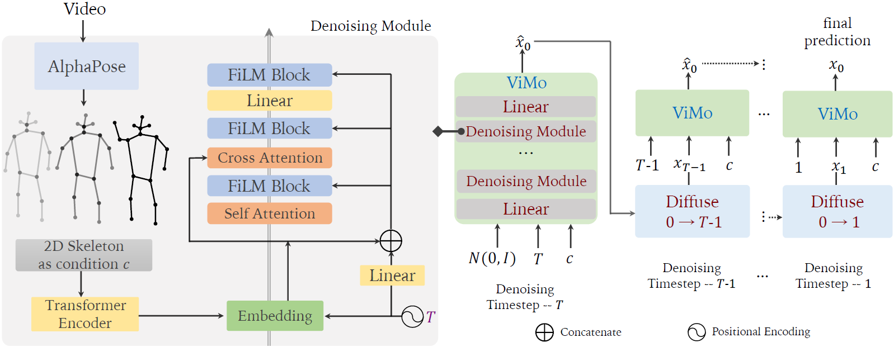
\includegraphics[width=\textwidth]{Pictures/vimo.png}
    \caption{ViMo denoising pipeline. Given a 2D pose sequence \(\mathbf{c}\), the model starts from noise \(\mathbf{m}_T\) and iteratively denoises \(\mathbf{m}_t\) for \(t = T \rightarrow 0\) to obtain a 3D motion sequence \(\mathbf{m}_0\), predicting the motion at each step while remaining robust to casual videos without explicit camera calibration.}
    \label{fig:vimo}
\end{figure}

The denoiser stacks three transformer blocks, each containing self-attention, cross-attention, and an MLP. The first self-attention block leverages the temporal context from the noisy motion input. Cross-attention conditions the model on 2D pose tokens, and FiLM blocks modulate intermediate activations using scale and shift parameters derived from the timestep and pose encoding. A final linear layer projects the output back to the motion space. The architecture is designed to gradually recover the data by reducing noise from time step $t$ to $t-1$ through these denoising modules.

Two FiLM strategies were examined:
\begin{itemize}
    \item Version~1 computes a single pair of gamma/beta parameters, shared across all three modulation points within each block. This approach reduces parameter count and enforces consistent conditioning across frames.
    \item Version~2 uses three separate linear layers within each block, generating distinct gamma/beta parameters for the self-attention, cross-attention, and MLP outputs respectively. This provides finer-grained control but increases the parameter count.
\end{itemize}
Both versions broadcast the same modulation parameters across all frames within a sequence, ensuring global consistency in the conditioning signal. Version~1 is more parameter-efficient and enforces a consistent style, while Version~2 offers more nuanced control at the cost of additional parameters.

\subsubsection{FiLM Conditioning}
Feature-wise Linear Modulation applies an affine transformation
\[
\mathbf{y}=\gamma(\mathbf{c})\odot\mathbf{x}+\beta(\mathbf{c})
\]
to intermediate activations $\mathbf{x}$, where $\gamma,\beta$ are generated from a condition vector $\mathbf{c}$~\cite{film2017}. This mechanism allows the network to dynamically rescale and bias feature channels based on external context. In this work, $\mathbf{c}$ is the concatenation of a timestep embedding $\text{embed}(t)$ and a pose-sequence encoding $\text{encode}(\mathbf{p})$. The encoding network processes the full 2D trajectory through a lightweight temporal transformer, producing a compact representation that captures pose shape and rhythm. FiLM then translates this representation into modulation parameters, aligning the denoising behavior with the input video.

\subsubsection{Sampling and Training Strategy}
Classifier-free guidance~\cite{vimo2024} is employed during both training and generation. The condition $\mathbf{p}$ is randomly dropped with probability 0.25, allowing the model to learn both conditioned and unconditioned distributions. 
At sampling, the final estimate combines both modes:
\[
\hat{\mathbf{m}}_0=(1+w)D(\mathbf{m}_t,t,\mathbf{p})-w D(\mathbf{m}_t,t,\varnothing),
\]
where $w$ controls adherence to the input versus diversity. 

\begin{figure}[htb]
    \centering
    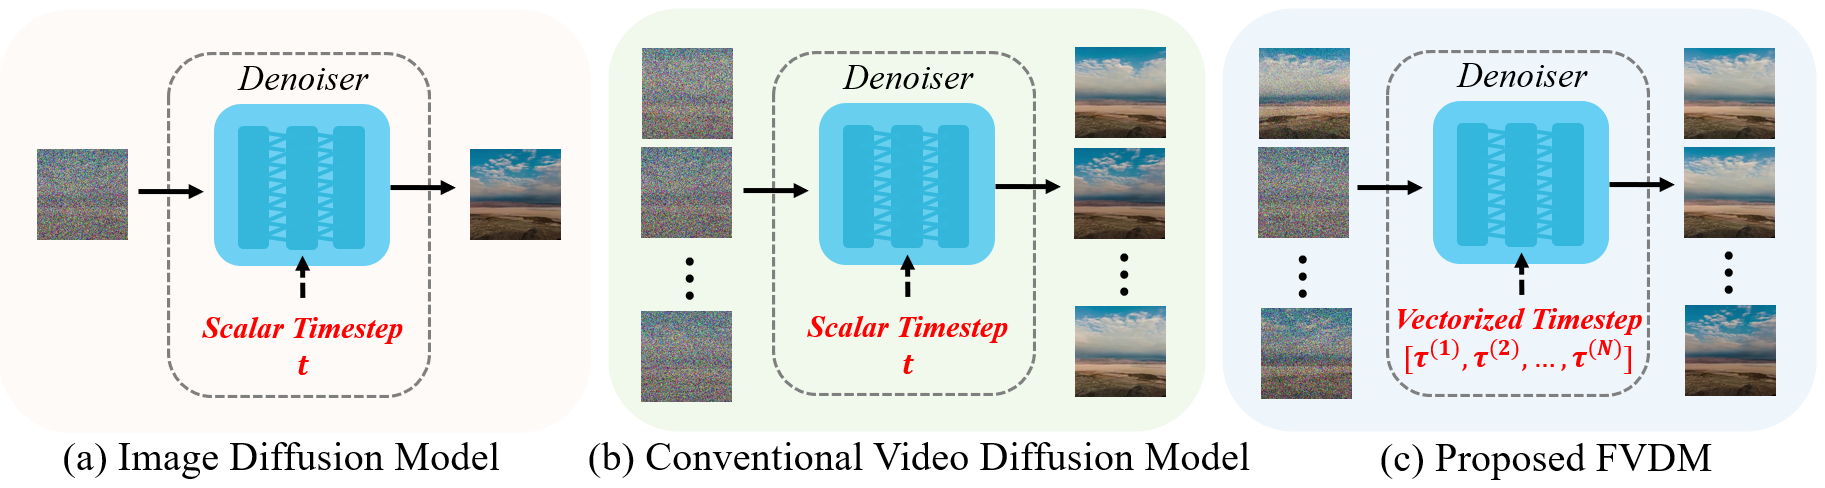
\includegraphics[width=\textwidth]{Pictures/fdvm.png}
    \caption{Previous conventional video diffusion models (b) directly extend image diffusion models (a) utilizing a single scalar timestep on the whole video clip. This straightforward adaption restricts the flexibilities of VDM’s in downstream tasks, e.g., image-to-video generation, longer video generation, (c). Frame-Aware Video Diffusion Model (FVDM~\cite{ptss2024}), which trains the denoiser via a vectorized timestep variable}
    \label{fig:fdvm}
\end{figure}

To prevent combinatorial explosion when using vectorized timesteps, PTSS~\cite{ptss2024} is introduced. With probability $p$, each frame receives an independently sampled timestep; otherwise, a single timestep is broadcast across all frames. This hybrid approach bounds the number of distinct schedules during training while preserving frame-wise temporal flexibility, stabilizing optimization without sacrificing rhythmic fidelity.